
\subsection{1. Mose 1 (Genesis 1)}
Das erste Kapitel gibt einen Überblick wie Gott das Universum (Verse: 1 - 5), die Wasser (Verse 6 - 10), die Pflanzen (Verse 11 - 13), die Tage ( Verse 14 - 19), die Tiere (Verse 20 -25) und die Menschen (Verse 26 - 27) geschaffen hat. Die Erschaffung des Menschen ist im 1 Kapitel relativ kurz gehalten. Diese wird dann im Kapitel 2 ausführlicher behandelt.

Jede Schöpfung geschieht an einem Tag. Am Ende des Tages heisst es immer: \begin{quote}
    Und es wurde Abend, und es wurde Morgen der fünfte Tag.
\end{quote} Das heisst der Tag hatte einen normalen Ablauf. Am Morgen aufstehen mit der Arbeit beginnen und am Abend die Arbeit niederlegen und ab in den Feierabend.

Es wird auch aufgezeigt, dass jeden Abend Gott sein Werk betrachtete und mit seiner Arbeit zu frieden war.

Ich finde das wir aus diesem Kapitel lernen können wie wir unsere Tage gestalten sollten. Am Tag die Arbeit verrichten und nach getaner Arbeit zufrieden auf diese zurückblicken. Es ist auch wichtig, dass wir wirklich in den Feierabend gehen und die Arbeit bis am Morgen wieder ruhen lassen.

Gott hat nicht alles an einem Tag erschaffen um der Rest der Woche frei zu haben. Es ist sehr wichtig, dass wir mit unserem Tag zufrieden sind. Als ehemaliger Bäcker weiss ich, dass die Nachtarbeit sehr anstrengend ist. Da ist es sehr wichtig, dass man sich die Erholung am Tag holt. Dies ist natürlich schwieriger, weil es hell und lauter ist.
\subsection{2. Mose (Genesis 2)}
Im zweiten Kapitel wird am Anfang der 7. Tag der Woche beschrieben. 
\begin{bibeltext}{Sch2}{Gen}{2:3}
    Und Gott segnete den siebten Tag und heiligte ihn, denn an ihm ruhte er von seinem ganzen Werk, das Gott schuf, als er es machte.
\end{bibeltext}
Hier steht ja nirgends, dass der siebte Tag ein Sonntag oder ein Sabbat war. Es heisst einfach, dass Gott nach 6 Tagen arbeiten, diese hingelegt hat. Am siebten Tag hat er geruht. Er ging nicht auf den neuen Meer Surfen, sondern er hat geruht. Welcher Tag das in der Woche ist finde ich unwichtig. Aber es sollte ein Tag in der Woche geruht werden.

An diesem Tag können wir einen Rückblick der Woche machen und Gott für seine Fürsorge danken. In unserem Arbeitssystem ist sicher gestellt, dass wir einen Tag frei haben. Öfters wird dieser Tag aber für einen andere Arbeit benutzt. Es gibt sicher Menschen denen das Geld von sechs Tage Arbeit, zum leben nicht reicht. Es geht aber nicht nur um die Existenz. Bei uns im Wallis war Sonntagsarbeit immer verpönt. Die Nachbarn haben darauf geachtet, dass man nicht Arbeit und zum Gottesdienst geht. Die jungen Bauern von heute kennen das nicht mehr. Die Woche auf der regulären Arbeit, am Wochenende dann auf der Wiese. Aber viele Hobbys arten zu Arbeit aus. Vor allem Sport Wettkampf. Das Training die Leistung alles braucht Substanz und man kommt nicht zur der Ruhe die man braucht um sich zu erholen.

In den restlichen Versen wird dann die Erschaffung des Menschen detaillierter aufgezeigt. Von 4 - 6 wird nochmals kurz die Schöpfung zusammengefasst und dann die Erschaffung den Menschen aus \flqq Staub von der Erde \frqq{}. 

Innerhalb seiner Schöpfung pflanzte Gott einen Garten und setzte den Menschen da hinein. In diesem Garten standen auch die zwei verhängnisvollen Bäume \flqq Baum des Lebens\frqq{} und \flqq Baum der Erkenntnis des Guten und Bösen\frqq{}. Dieser Garten wird der Garten Eden genannt. In diesem Garten lebte der Mensch mit Gott zusammen. Gott hat die Angewohnheit am Abend in Eden spazieren zu gehen. Gott gab aber dem Menschen die Anweisung, dass er die Früchte von dem \flqq Baum der Erkenntnis des Guten und Bösen\flqq{}, nicht essen darf.
\begin{bibeltext}{Sch2}{Gen}{2:17}
	aber von dem Baum der Erkenntnis des Guten und des Bösen sollst du nicht essen; denn an dem Tag, da du davon isst, musst du gewisslich sterben!\footnote{Die ersten Menschen kannten den Tod noch nicht; er kam erst als Folge der Sünde über den Menschen. \bibleverse{Rom} {5:12}; \bibleverse{Rom} {6:23}; \bibleverse{Eph} {2:1-3}}
	Inhalt...
\end{bibeltext}
Ab Vers 18 kommen wir zur Erschaffung der Frau. Nachdem der erste Mensch allen Tieren einen Namen gegeben hat und herausgefunden hatte, dass unter den Tieren kein wirklich gegenüber zu finden war, hat Gott aus der Rippe des ersten Menschen die Frau erschaffen. 
\begin{bibeltext}{Sch2}{Gen}{2:24}
	Darum wird ein Mann seinen Vater und seine Mutter verlassen und seiner Frau anhängen.	
\end{bibeltext}
Ein interessanter Satz. Das zeigt mir, dass diese ersten beiden Menschen auch im Garten Eden Kinder bekommen hätten und diese dann später geheiratet hätten. Oder der Autor hat diesen Satz hinzugefügt, um die heutige Hochzeit zwischen Mann und Frau zu erklären. In jeder Kultur werden die Paare verheiratet. Irgend wie hat das Heiraten was. Wieso wollen gleichgeschlechtliche Paare eigentlich immer heiraten? Wieso reicht es ihnen nicht einfach zusammen zu leben? Gesetzlich könnte man das ja einfach regeln. Es muss etwas im Menschen sein das diesem das Bedürfnis gibt, dass eine höhere Instanz die Zustimmung zu dem zusammenleben gibt.

Das Kapitel 2 hat einen sehr schönen Abschluss:
\begin{bibeltext}{Sch2}{Gen}{2:25}
	Und sie waren beide nackt, der Mensch und seine Frau, und sie schämten sich nicht.
\end{bibeltext}
\subsection{1. Mose 3 (Genesis 3)}
In diesem Kapitel wird der Sündenfall des Menschen beschrieben. Die Geschehnisse in diesem Kapitel sind der Grund wieso die Bibel Überhaupt geschrieben werden musste. Nach dem Sündenfall des Menschen, musste Gott den ganzen Heilsplan in Bewegung setzten, um die Menschen wieder in seine Nähe zu ziehen.

Es ist erstaunlich, dass schon diese zwei Menschen schon daran interessiert waren, Macht zu besitzen. Eigentlich ging es doch ihnen gut im Paradies. Hatten alles, aber trotzdem wollten sie mehr. Sie wollten so sein wie Gott. Die Schlange hat es ihnen versprochen. Sie müssen nur von diesem Baum essen.
\begin{bibeltext}{Sch2}{Gen}{3:1}
	Aber die Schlange war listiger als alle Tiere des Feldes, die Gott der Herr gemacht hatte; und sie sprach zur Frau: Sollte Gott wirklich gesagt haben, dass ihr von \textbf{keinem} Baum im Garten essen dürft?
\end{bibeltext}
Das hat doch die Schlange geschickt eingefädelt oder? Sie macht der Frau den Mund richtig wässrig. Kann doch nicht so schlimm sein. Gott will euch doch etwas vorenthalten. \flqq Ihr werdet sein wie Gott... \frqq{}. Wollen wir das nicht auch heute noch? Sein wie Gott? Flüstert der Satan uns nicht immer noch ins Ohr, \flqq Hat er euch wirklich diese strengen Gebote gegeben? Hat Gott verboten Spass zu haben? Er ist doch ein Spielverderber. Hört nicht auf ihn. Ihr seid viel schlauer als er. Mit der Wissenschaft seid ihr die Götter.\frqq{} 
Nachdem beide von dem tollen Baum gegessen haben geschieht es. \flqq \textbf{Da erkannten sie dass sie nackt waren...} \frqq{}. Ende letztes Kapitel heisst es: \flqq und sie waren nackt und schämten sich nicht\frqq{}. Das ist die Erkenntnis von Gut und Böse. Jetzt sieht der Mensch das Böse vom anderen. Sie schämten sich vor einander, sie konnten sich gegenseitig nicht mehr in die Augen blicken.\\
Als dann Gott sie suchte versteckten sie sich im Garten. Das Raus reden ist typisch für uns Menschen. Der Mann schiebt die Verantwortung auf die Frau und auf Gott. \flqq Du hast mir die Frau gegeben \frqq{}. Die schiebt die Schuld auf die Schlange. Also genau so wie wir uns noch Heute aus der Verantwortung winden wollen.

Diese Aktion hatte weitreichende Auswirkungen die wir noch heute spüren. Es kam der Tod, der Schmerz in die Welt. Die Auswirkungen waren so schlimm, dass Gottes Plan schon zu dieser Zeit festgelegt war, seinen Sohn für die Erlösung von uns Menschen zu schicken. Die Menschheit musste aber zuerst vorbereitet werden. Hier tauchen die ersten Hinweise auf das Opfer von seinem Sohn. So sagt Gott zu der Schlange:
\begin{bibeltext}{Sch2}{Gen}{3:15}
	Und ich will Feindschaft setzten zwischen dir und der Frau, zwischen deinem Samen und ihrem Samen: Er wird dir den Kopf zertreten, und du wirst ihn in die Ferse stechen.
\end{bibeltext}
Hier wird gezeigt wie Jesus den Satan besiegt, \flqq er wird ihm den Kopf zertreten, mit flqq in die Ferse steche \frqq{} meint die Kreuzigung Jesus. Im weiteren Verlauf der Bibel werden die Hinweise auf Jesus immer konkreter.
Auch die beiden Menschen bekamen ihre Strafe, mit der wir noch jetzt leben und zu kämpfen haben. Geburtsschmerzen, Krankheit auch die strenge Arbeit zum überleben, hat von an ihren Anfang.

Adam\footnote{Hebr. Adama: Erdboden. Dient als Eigennamen für den Mensch} nannte seine Frau Eva\footnote{Hebr. Chawa: Leben} und Gott stattete die beiden mit Kleider aus Fellen aus. Die Auslegung sagt, dass die Felle das erste Blutopfer für die begangene Sünde des Menschen war. Dar letzte Blutopfer hat Jesus der Christus für uns am Kreuz in Golgotha vollbracht.
\subsection{1. Mose 4 (Genesis 4)}
Eva wurde schwanger und gebar den Kain\footnote{bed. Erwerb}. Später gebar sie einen zweiten Sohn mit dem Namen Abel. Ich glaube das ist das berühmteste Pärchen auf dieser Welt. Kain und Abel. Es heisst hier, Kain war Ackerbauer und Abel ein Schafhirte. Beide brachten dem Herrn ein Opfer dar. Kain von den Früchten der Erde und Abel schlachtete ein Schaf. Gott sah das Opfer von Abel an aber das von Kain nicht. War es wirklich nur darum, dass Kain kein Tier geschlachtet hat? Ich kann das nichst so recht glauben. Kann es nicht auch sein, dass Kain schon immer ein Problemkind war? Als Gott sein Opfer nicht anerkannte, wurde er ja ziemlich zornig auf seinen Bruder. Wenn ich ohne Gott unterwegs bin und gegen ihn sündige, wird es wohl nicht reichen wenn ich ihm einfach ein Opfer darbringe und denke, jetzt ist er wieder zufrieden mit mir. Als er dann sah dass es doch nicht so einfach ist Gott zu beeinflussen, wurde er dann halt sauer. Gott ihn ja darauf aufmerksam gemacht. Er hätte es vor Gott wieder gutmachen können.
\begin{bibeltext}{ELB}{Gen}{4:6-7}
	Und der \herr{} sprach zu Kain: "Warum bist du ergrimmt, und warum und warum hat sich dein Angesicht gesent? Ist es nicht so, dass es sich erhebt, wenn du recht tust?"
\end{bibeltext}
Das ist doch etwas was uns auch immer wieder passiert. Wenn wir merken, dass wir etwas schlimmes getan haben, ducken wir uns und wir dürfen nicht mehr direkt in die Augen schauen? Da gibt es dann Zwei Möglichkeiten, wir biegen das geleistete wieder gerade und bringen es vor Gott oder wir kehren es unter den Tisch und warten bis sich alles als Hass in uns aufgestaut hat. Man wird bitter und wird böse gegenüber der Umwelt. Wer jetzt eher Gewalttätig ist lässt es an anderen raus oder er tut sich selber Gewalt an. Kain ging dann in die grosse weite Welt und gründete dort eine Stadt. Die Nachkommen Kain gründeten die Zivilisation. Adam bekam noch einen weiteren Sohn. Diese Sohn nannte er Set. Aus der Linie Set entstammte Noah.

\subsection{1. Mose 5 (Genesis 5)}
In diesem Kapitel wird das Geschlechtsregister Adams bis Noah aufgelistet. Die Menschen wurden zu der Zeit ziemlich alt. Durch dieses Alter gab es eine Spezielle Konstellation.
\begin{figure}[htb]
	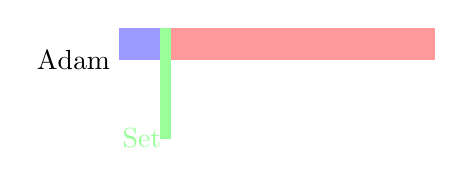
\begin{tikzpicture}
		\filldraw[blue!40] (0,0) node[black][left]{Adam} rectangle(.65,.4);
		\filldraw[red!40] (.65,0) rectangle(4,.4);
		\filldraw[green!40] (.65,-1) node[left]{Set} rectangle(.525,.4);
	\end{tikzpicture}				
\end{figure}





